\chapter{Un tour de C}
\thispagestyle{empty}

%% Calculate how old C is...
\newcount\cdifference\cdifference=\the\year\advance\cdifference by -1970

C is al een oude taal. De taal is rond 1970 ontworpen door Dennis Ritchie\footnote{Dennis MacAlister Ritchie (1941 -- 2011). Hij was de ontwerper van de programmeertaal C en was een van de ontwerpers van Unix. Bekende afgeleiden van Unix zijn Linux en FreeBSD.} en is dus al zo'n \the\cdifference\ jaar oud. Hij was bezig met het schrijven van een Operating System en zocht naar een mogelijkheid om dit te schrijven op een hoger niveau dat gebruikelijk voor die tijd. In die tijd werden operating systems geschreven in assembly, een taal die dicht de hardware van de computer ligt. Programma's schrijven in assembly is tijdrovend en gevoelig voor fouten van de programmeur.

C is een zogenoemde derde-generatie-taal (3GL) en zorgt ervoor dat programm's gestructureerd kunnen worden geschreven zonder dat de programmeur kennis hoeft te hebben van de hardware waarop het programma draait. Toch biedt de taal contructies om die hardware in te stellen, een voorwaarde voor het schrijven van een operating system. Daarom is de taal geliefd bij programmeurs van kleine computersystemen waarop geen operating system draait, de zogenoemde \textsl{bare metal systems}. Het is vaak ook de enige taal die gebruikt kan worden op dit soort systemen, naast assembly.

C is geschreven voor ervaren programmeurs die behoefte hebben voor het schrijven van compacte programma's, dat te zien is in de vele, soms onduidelijke, taalconstructies. Het is eigenlijk niet geschikt voor beginnende programmeurs. Het is zeker mogelijk om programma's te schrijven die niet correct werken, maar met enige discipline kan ook de minder ervaren programmeur de taal prima gebruiken.

C is een algemeen bruikbare taal (\textsl{general purpose language}) en is dus niet voor een specifiek doeleind ontworpen (behalve voor het schrijven van operating systems). Zo kunnen met C wiskundige berekeningen worden uitgevoerd maar de programmeur moet zelf alles schrijven. Er zijn wel \textsl{functies} beschikbaar voor bijvoorbeeld sinus, cosinus en tangens. Er zijn echter talen die dit veel beter ondersteunen. Ook het verwerken van bestanden is mogelijk maar het manipuleren van \textsl{strings} (een rij karakters) moet door de programmeur zelf worden uitgewerkt. Ook hier zijn diverse functies beschikbaar die het programmeerwerk enigszings verlichten.

C is een \textsl{imperatieve} programmeertaal, een van de bekende programmeerparadigma's\footnote{Een programmeerparadigma is een manier van programmeren en een wijze waarop een programma wordt vormgegeven.}
C moet concurreren met vele andere talen zoals C++, C\#, Python en Java. C++ is ontwikkeld door Bjarne Stroustrup als ``de betere C'' en ondersteunt \textsl{objectgeoriënteerd} programmeren. C\# is ontwikkeld door MicroSoft en is de \textsl{de facto} programmeertaal op Windows-systemen. Python is ontwikkeld door het Centrum voor Wiskunde en Informatica van de Universiteit van Amsterdam. 

\section{Ontwikkelsystemen}
De meeste boeken gaan uit van een \textsl{command line interface} op een Unix-derivaat. Met behulp van een \textsl{editor} wordt een programma ingevoerd en wordt op de commandoregel de C-compiler gestart. Daarna wordt het programma (ook via de commandoregel) gestart. Deze werkwijze kan ook op Windows worden gebruikt. Een voorbeeld is te zien in onderstaande figuur.

\begin{dosbox}
C:\textbackslash Users\textbackslash C> notepad opdracht.c \hfill\textrm{(start Notepad)} \\
C:\textbackslash Users\textbackslash C> gcc -o opdracht.exe opdracht.c \hfill\textrm{(start C-compiler)}\\
C:\textbackslash Users\textbackslash C> .\textbackslash opdracht.exe \hfill\textrm{(start uitvoerbaar programma)}\\
C is een mooie taal \\
C:\textbackslash Users\textbackslash C>
\end{dosbox}

Dit is echter niet de werkwijze van veel programmeurs. Gelukkig zijn er goede ontwikkelsystemen (IDE: Integrated Development Environment) die het programmeerwerk verlichten. Bekende systemen zijn Microsoft Visual Studio en Code::Blocks.

Een voorbeeld van Microsoft Visual Studio is te zien in figuur~\ref{fig:unvs2019}. Visual Studio ondersteunt het ontwikkelen van software voor Windows-computers met behulp van een groot aantal talen: C, C++, C\#, Python. Het is zelfs mogelijk om software te ontwikkelen voor Linux-systemen.



\begin{figure}[H]
\centering
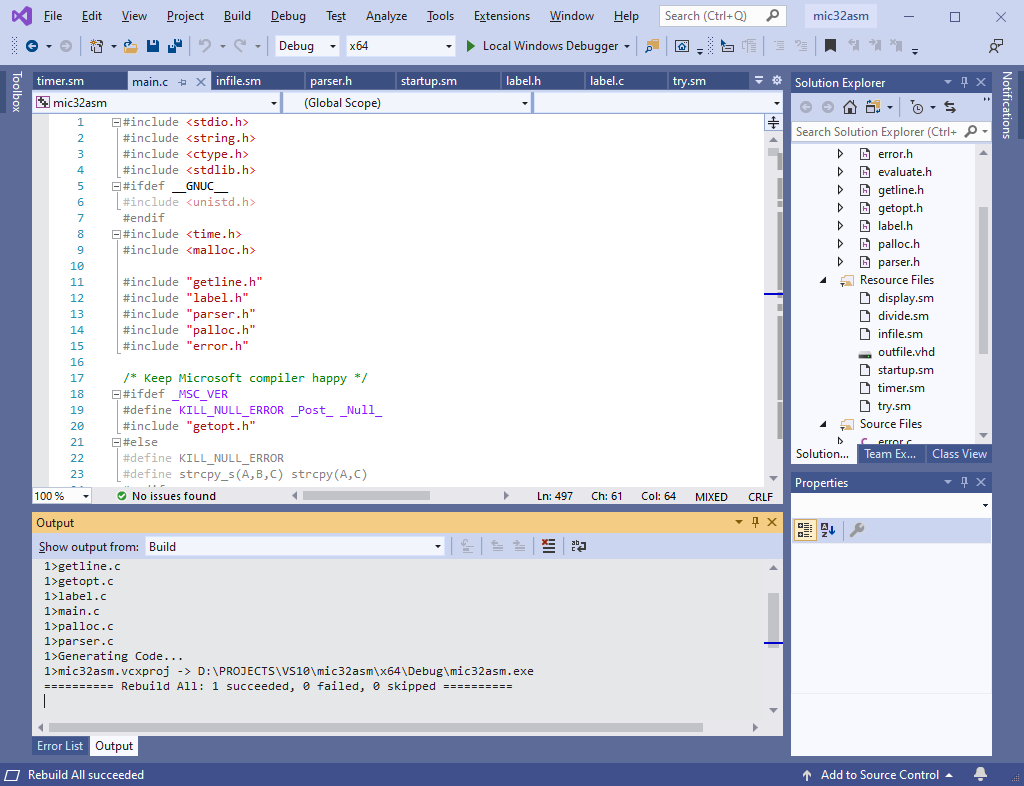
\includegraphics[scale=\figscale]{images/vs2019}
\caption{Voorbeeld van Microsoft Visual Stdio.}
\label{fig:unvs2019}
\end{figure}

\section{Eerste programma}
Laten we beginnen met een eenvoudig voorbeeld. Het programma in listing~\ref{cod:uneersteprogramma} drukt de regel \texttt{C is een mooie taal} op het scherm af. We zullen het programma stap voor stap doorlopen.

\begin{lstlisting}[caption=Eerste C-programma.,label=cod:uneersteprogramma]
#include <stdio.h>

int main(void) {

	printf("C is een mooie taal\n");
	return 0;
}
\end{lstlisting}
